\documentclass[xcolor={dvipsnames}]{beamer}

% Variable "animation" : = 1   --> animations   (avec \animategraphics)
%                        sinon --> images fixes (avec \includegraphics)
\def \animation {0}

% Paquets utilisés
\usepackage{animate} % pour faire des animations
\usepackage{listings} % pour insérer des lignes de codes avec de la coloration syntaxique
\usepackage[audience=french]{beameraudience}  % pour écrire la présentation en 2 langues
\usepackage{textpos} % pour positionner des figure où l'on veut
\usepackage{tikz} % pour faire de jolies figures
\usepackage{pifont} % pour avoir des symboles sympa

% Thème et options générales de mise en forme
\usetheme{Singapore}
\usecolortheme{rose}
\setbeamertemplate{page number in head/foot}[totalframenumber] % pour ajouter les numéros des pages
\setbeamertemplate{navigation symbols}{} % pour virer les symboles "page suivantes" ...
\makeatletter % pour avoir des puces de progression
\setbeamersize{
  text margin left = 0.2cm, % modification des marges (normalement c'est 1 cm)
  text margin right = 0.2cm}
\setbeamertemplate{block begin}{  % pour ajuster la taille des block
  \begin{minipage}{.87\textwidth}%
    \begin{beamerboxesrounded}[upper=block title,lower=block body,shadow=true]{
    \raggedright\usebeamerfont*{block title}\insertblocktitle}
    \raggedright
    \usebeamerfont{block body}}
  \setbeamertemplate{block end}
{\end{beamerboxesrounded}\end{minipage}\vskip\smallskipamount}
\setlength{\unitlength}{1cm}

% Ajout de la description du language Gibiane (pour le paquet "listings")
\lstdefinelanguage{gibiane}{
  morekeywords=[1]{
      opti, born, dens, droi, lapl, cerc, mota, oper,
      quel, inte, para, et  , poin, plus, moin, tran, lister,
      rota, trac, inve, cote, elem, cont, diff, chan, list,
      surf, conf, info, tour, homo, affi, syme, incl, elim,
      titr, racc, tass, sort, lire, bary, dall, orie, manu,
      oubl, comp, cout, pave, comm, noeu, mot , nbel, nbno,
      noti, face, coor, norm, temp, volu, lect, sauf, prog,
      +   , -   , *   , /   , **  , flot, enti, log , exp ,
      depl, psca, pvec, pmix, liai, regl, hook, sols, reso,
      date, rigi, bloq, depi, hota, stru, text, proj, venv,
      elst, jonc, reco, mass, clst, sigm, rela, forc, mome,
      vloc, base, dime, extr, vers, vibr, maxi, xtmx, ytmx,
      >   , <   , >eg , <eg , ou  , ega , non , neg , mult,
      pjba, crit, diag, xtx , uniq, bsig, deda, max1, mots,
      ipol, abs , sin , cos ,
      atg , enve, isov, detr, enle, remp, inse, coli, tria,
      tabl, redu, symt, anti, resu, pres, exco, nomc, saut,
      defo, appu, inva, prin, vmis, ksig, sign, suit, 
      valp, ordo, tire, rege, dess, amor, char, coul, chpo,
      afco, evol, orth, thet, comb, deve, vect, pica, capi, 
      copi, dimn, sauv, rest, cara, mate, gene,
      capa, elfe, jaco, plas, gree, mode, finp, xty ,
      debp, ktan, form, mess, nnor, cubp, cubt, cer3, fdt ,
      seis, ener, epsi, intg, cour, reac, supe, zero, depb,
      exci, kp  , acti, elas, erre, cong, lump, obte,
      vari, modi, masq, exis, mini, grad, ense, ifre, dfou,
      sigs, mapp, somm, brui, rten, dspr, tfr , tote,
      graf, tres, type, osci, spo , inde, chsp,
      tagr, perm, cabl, fofi, work, qulx, debi, 
      cmoy, comt, cond, flux, rimp, filt, tfri,
      conc, iter, acqu, sour, conv, acoh, psmo, asih, ecou,
      mena, synt, argu, atah, dyne, fonc, resp, plac,
      vale, proi, exce, aret, calp, indi, act3, biot,
      dedu, conn, nloc, chai, cosi, cvol, diad, hann, insi,
      lsqf, ltl , pert, prns, psrs, siar, spon, visa, cneq,
      ccon, mesu, pile, simp, util, menu, cosh, sinh, tanh,
      deg3, aide, racp, refe, ksof, nske, kmab,
      noel, doma, fpu , gmv , eqpr, eqex, vibc, avct,
      kdia, kmtp, kmf , mdia, dfdt, tcrr, tcnm, sqtp, somt,
      nlin, cmct, kcht, lapn, raft, klop, kres, cson, fimp, 
      nuag, weip, khis, kops, fsur, flam, elno,
      dbit, ns  , toim, fimp, kmbt, kbbt, dudw, frot, tsca,
      konv, kcha, mhyb, matp, hdeb, hvit, hybp, smtp, divu,
      mocu, chau, tail, erf , sens, impo, dans, impf, ntab,
      fron, fuit, epth, fpt , kfpt, fpa , kfpa, echi, qond,
      kpro, ffor, raye, rayn, vsur, traj, aju1, aju2, frig,
      excf, nomm, prec, erfc, onde, cfl , dedo, dcov, parc,
      pola, chi1, chi2, pent, pret, meth, xxt , cblo, genj,
      zleg, mesm, fion, neut, logk, coac, resi, mutu, sore,
      diri, lign, obje, debm, finm, heri, deco, exte, dmmu,
      dmtd, bmtd, ssch, mrem, assi, fiss, prim, annu, prob,
      sais, choi, deto, part, clmi, pmat, excp, prop, phaj,
      alea, gnfl, mpro, sste, adve, bgmo, ecfe, coup, verm,
      dfer, gyro, cori, kent, fant, itrc, reto, ijet, impe,
      moca, levm, ravc, idli, raff, cfnd, adet, psip, acos,
      asin, tan , trie, gane, hist, etg , oter, xfem, rfco,
      vide, voro, prra, posi, mise, misl, coll, pod,  
      option, borne, droit, droite, point, moins, titre,
  },
  morekeywords=[2]{  % quelques procedures
    pasapas, peche, explorer
  },
  morekeywords=[3]{  % operateurs speciaux
    si, sino, sinon, fins, finsi, repe, repeter, quit, fin
  },
  sensitive=false, % mots clefs non sensibles à la casse
  morecomment=[f]*, % indique que les commentaires ont des * en 'first' colonne
  morestring=[b]', % indique que les chaines sont définies entre simples quotes
  moredelim=[is][\sffamily\slshape\color{blue}]{/*}{*/}
}
\definecolor{bckg}{rgb}{0.96,0.96,0.96}
\lstset{
%  language={gibiane},
%  backgroundcolor=\color{white},
  keywordstyle=[1]\color{red}\bfseries,
  keywordstyle=[2]\color{orange}\bfseries,
  keywordstyle=[3]\color{blue}\bfseries,
  commentstyle=\color{Aquamarine},
  stringstyle=\color{Green},
  basicstyle=\ttfamily\scriptsize,
  %captionpos=b, % Position of the Caption (t for top, b for bottom)
  %extendedchars=true, % Allows 256 instead of 128 ASCII characters
  tabsize=2, % number of spaces indented when discovering a tab 
  columns=fixed, % make all characters equal width
  keepspaces=true, % does not ignore spaces to fit width, convert tabs to spaces
  showstringspaces=false, % lets spaces in strings appear as real spaces
  breaklines=true, % wrap lines if they don't fit
  %frame=tb, % draw a frame at the top, right, left and bottom of the listing
  %frameround=tttt, % make the frame round at all four corners
  %framesep=4pt, % quarter circle size of the round corners
  %framexleftmargin=2mm, framexrightmargin=2mm,
  %framextopmargin=2mm,framexbottommargin=2mm,
  %frame=shadowbox, rulesepcolor=\color{gray},
  xrightmargin=5mm,
  belowskip=0pt
}


% Infos générales : titre / sous titre / date / auteur / organisme ...
\justfor{french}{
  \title{Débuter avec Cast3M}
  \subtitle{calculs thermo mécaniques}
  \date{Été 2024}}
\justfor{english}{
  \title{Starting with Cast3M}
  \subtitle{thermomechanical calculations}
  \date{Summer 2024}}
\author{François Di Paola}
\institute{CEA Saclay,\\
\url{https://www-cast3m.cea.fr}}

% Quelques raccourcis perso
\newcommand{\fe}[2]{\justfor{french}{#1}\justfor{english}{#2}}
\newcommand{\g}[1]{\textbf{#1}}
\newcommand{\tou}[1]{\underline{#1}}
\newcommand{\tod}[1]{\underline{\underline{#1}}}
\newcommand{\kw}[1]{\mbox{\texttt{#1}}}
\newcommand{\kwr}[1]{\textcolor{red}{\kw{#1}}}
\newcommand{\kwg}[1]{\textcolor{Green}{\kw{#1}}}
\newcommand{\kwo}[1]{\textcolor{orange}{\kw{#1}}}
\newcommand{\kwb}[1]{\textcolor{blue}{\kw{#1}}}
\newcommand{\red}[1]{\textcolor{red}{#1}}
\newcommand{\orange}[1]{\textcolor{orange}{#1}}
\newcommand{\green}[1]{\textcolor{Green}{#1}}
\newcommand{\blue}[1]{\textcolor{blue}{#1}}
\newcommand{\violet}[1]{\textcolor{violet}{#1}}
\newcommand{\gray}[1]{\textcolor{gray}{#1}}
\newcommand{\white}[1]{\textcolor{white}{#1}}
\newcommand{\grille}{\draw[help lines,xstep=.1,ystep=.1] (0,0) grid (1,1);
                     \foreach \x in {0,1,...,9} { \node [anchor=north] at (\x/10,0) {0.\x}; }
                     \foreach \y in {0,1,...,9} { \node [anchor=east] at (0,\y/10) {0.\y}; }}
\newcommand{\avous}[1]{\orange{\ding{43}\emph{#1}}}
\newcommand{\tx}[1]{\textsf{#1}}


\begin{document}

\begin{frame}
  \titlepage
\end{frame}

\begin{frame}{\fe{Sommaire}{Summary}}
  \begin{itemize}
    \item \fe{\hyperlink{presentation}{Présentation de Cast3M}}
             {\hyperlink{presentation}{Introduction to Cast3M}}
    \item \fe{\hyperlink{gibiane}{Le langage Gibiane}}
             {\hyperlink{gibiane}{Gibiane language}}
    \item \fe{\hyperlink{maillage}{Travaux dirigés}}
             {\hyperlink{maillage}{Tutorial class}}\\
          \begin{center}
            \fe{\hyperlink{thermique}{\emph{Thermo}} \hyperlink{mecanique}{\emph{mécanique}} \emph{d'une structure avec un trou}}
               {\hyperlink{thermique}{\emph{Thermo}} \hyperlink{mecanique}{\emph{mechanical}} \emph{behavior of a structure with a hole}}\\
          \includegraphics[height=0.242\textheight]{images/exo/1.2_maillage_hexa.4} \hspace{2mm}
          \includegraphics[height=0.275\textheight]{images/exo/2.1_temperatures.3}  \hspace{2mm}
          \includegraphics[height=0.275\textheight]{images/exo/8_contraintes}
          \end{center}
    \item \fe{\hyperlink{complements}{Compléments}}
             {\hyperlink{complements}{Complements}}
  \end{itemize}
\end{frame}

%%%%%%%%%%%%%%%%%%%%%%%%%%%%%%%%%%%%%%%%%%%%%%%%%%%
\fe{\section{Présentation}}{\section{Presentation}}
\label{presentation}
%%%%%%%%%%%%%%%%%%%%%%%%%%%%%%%%%%%%%%%%%%%%%%%%%%%

\begin{frame}{\fe{Cast3M, quid ?}{What is Cast3M?}}
  \fe{Logiciel de simulation utilisant la \g{méthode des éléments finis} en \g{mécanique/thermique} des \g{structures} et des \g{fluides}}
     {A simulation software using the \g{finite element method} in \g{thermal and mechanical} analysis of \g{structures} and \g{fluids}}\pause
  \begin{itemize}
    \item \fe{Résolution d'\g{équations aux dérivées partielles}}
             {\g{Partial differential equations} solver}\pause
    \item \fe{\g{Système complet} : solveur, pré/post-processeur, visualisation, import/export des données\dots}
             {\g{Complete software}: solver, pre-processing and post-processing, visualization, reading/writing data\dots}\\
            ~\\
            \begin{center}
            \includegraphics[height=0.25\textheight]{images/plaque.1} \:
            \includegraphics[height=0.25\textheight]{images/plaque.2} \:
            \includegraphics[height=0.25\textheight]{images/plaque.3}
            \end{center}\pause
    \item \fe{Basé sur un langage de commande : \g{Gibiane} (orienté objet)}
             {Based on a programming language: \g{Gibiane} (objet-oriented)}\\
  \end{itemize}
\end{frame}

\begin{frame}{\fe{Nombreux domaines d'application}{Wide range of applications}}
  \small{
  \begin{itemize}
    \item<1->\fe{Mécanique des structures}{Structural mechanics}\\
    \footnotesize{
      \fe{\red{Quasi-statique} (non linéarités matériau, géométrie, conditions limites)}
         {\red{Quasi-static} (non linear behavior, geometry, boundary conditions)}\\
      \onslide<1>{
        \begin{textblock*}{5cm}(2cm,0.3cm)
          \includegraphics[height=0.4\textheight]{images/polycristal}
        \end{textblock*}
        \begin{textblock*}{5cm}(5cm,1.2cm)
          \includegraphics[height=0.4\textheight]{images/ressort}
        \end{textblock*}
        \begin{textblock*}{5cm}(8cm,2.1cm)
          \includegraphics[height=0.4\textheight]{images/galatee}
        \end{textblock*}
        \begin{textblock*}{5cm}(9.4cm,5.6cm)
          \tiny{\emph{(S. Durand)}}
        \end{textblock*}}
      \onslide<2->\fe{\orange{Contact/frottement}, \green{Flambage}}
                     {\orange{Contact/friction}, \green{Buckling}}\\
      \onslide<2>{
        \begin{textblock*}{5cm}(1cm,0.3cm)
          \includegraphics[height=0.25\textheight]{images/sac_a_dos.15}
        \end{textblock*}
        \begin{textblock*}{5cm}(4.8cm,0.3cm)
          \includegraphics[height=0.25\textheight]{images/sac_a_dos.32}
        \end{textblock*}
        \begin{textblock*}{5cm}(8.5cm,0.3cm)
          \includegraphics[height=0.25\textheight]{images/sac_a_dos.41}
        \end{textblock*}}
      \onslide<3->\fe{\blue{Dynamique} (temporelle, modale, interaction fluide structure)}
                     {\blue{Dynamic} (temporal, modal, fluid structure interaction)}\\
      \onslide<3>{
        \begin{textblock*}{5cm}(1cm,0.3cm)
          \includegraphics[height=0.2\textheight]{images/cymbale_mode_1}
        \end{textblock*}
        \begin{textblock*}{5cm}(4.8cm,0.3cm)
          \includegraphics[height=0.2\textheight]{images/cymbale_mode_2}
        \end{textblock*}
        \begin{textblock*}{5cm}(8.5cm,0.3cm)
          \includegraphics[height=0.2\textheight]{images/cymbale_mode_4}
        \end{textblock*}}
      \onslide<4->\fe{\violet{Rupture} (XFEM, propagation dynamique, zones cohésives)}
                     {\violet{Fracture} (XFEM, dynamic propagation, cohesive zones models)}\\
      \onslide<4>{
        \begin{textblock*}{12cm}(1.5cm,0.3cm)
          \includegraphics[height=0.25\textheight]{images/rousselier_03}
          \includegraphics[height=0.25\textheight]{images/rousselier_04}
          \includegraphics[height=0.25\textheight]{images/rousselier_05}
          \includegraphics[height=0.25\textheight]{images/rousselier_06}
          \includegraphics[height=0.25\textheight]{images/rousselier_07}
          \includegraphics[height=0.25\textheight]{images/rousselier_08}
        \end{textblock*}
        \begin{textblock*}{5cm}(8cm,4.7cm)
          \tiny{\emph{(S. Kebiri)}}
        \end{textblock*}}
      \onslide<5>{
        \begin{textblock*}{12cm}(4cm,1.3cm)
          \includegraphics[height=0.4\textheight]{images/te_temperature}\;
          \includegraphics[height=0.4\textheight]{images/te_sigma}
        \end{textblock*}}
      \onslide<6>{
        \begin{textblock*}{12cm}(6.5cm,1.2cm)
          \includegraphics[height=0.4\textheight]{images/metallurgie}
        \end{textblock*}
        \begin{textblock*}{5cm}(8cm,4.7cm)
          \tiny{\emph{(C. Berthinier)}}
        \end{textblock*}}
    }
    \item<5->\fe{Thermique}{Thermal analysis}\\
    \footnotesize{
      \fe{Conduction, convection, rayonnement, changement de phase}
         {Conduction, convection, radiation, phase transition}
    }
    \item<6->\fe{Mécanique des fluides}{Fluid mechanics}
    \item<6->\fe{Magnétostatique}{Magneto-statics}
    \item<6->\fe{Diffusion multi espèces (loi de Fick)}{Multi species diffusion (Fick’s law)}
    \item<6->\fe{Métallurgie}{Metallurgy}
  \item<6->\fe{Couplage thermo-hygro-mécanique}{Thermo-hygro-mechanics coupling}
  \end{itemize}
  }
\end{frame}

\begin{frame}{\fe{Comment obtenir Cast3M ?}{How to get Cast3M}}
  \begin{itemize}
    \item \fe{Multi plateformes}{Cross platform}\\
    \footnotesize
    \blue{Windows}, \red{Linux}, \green{macOS}
    \normalsize
    \item \fe{Où télécharger Cast3M ?}{Where can I download Cast3M?}\\
    \footnotesize
    \url{http://www-cast3m.cea.fr/index.php?page=dlcastem}
    \normalsize
    \item \fe{Accès au code source}{Access to the source code}\\
    \footnotesize
    \fe{Développement communautaire}{Open collaboration}\\
    \fe{Compilateur / éditeur de liens fournis}{Compiler / Linker are provided}
    \normalsize
    \item \fe{Prix}{Price}\\
    \footnotesize
    \fe{\green{Gratuit} pour la recherche et l’enseignement\\
        \red{Payant} pour une utilisation commerciale}
       {\green{Free} license, for education and research use\\
        \red{Paid} license, for enterprise use}
    \normalsize
    \item \fe{Utilisateurs/clients}{Users/customers}\\
    \footnotesize
    \fe{Universités, écoles d’ingénieurs\\
        IRSN, EDF, SNCF, CNRS, Framatome, Air Liquide, CERN, \dots}
       {Universities, engineering schools\\
        IRSN, EDF, SNCF, CNRS, Framatome, Air Liquide, CERN, \dots}\\
    \scriptsize
    \fe{Outil de référence IRSN pour les analyse de sureté des installations nucléaires françaises\\
        Outil de référence Framatome pour l’analyse en mécanique de la rupture}
       {Reference FEM tool for IRSN for safety analysis of French nuclear installations\\
        Reference tool for Framatome for fracture mechanics}
    \normalsize
    \end{itemize}
\end{frame}

\begin{frame}{\fe{Comment utiliser Cast3M ?}{How to launch Cast3M?}}
  \begin{textblock*}{5cm}(7.9cm,0cm)
    \animategraphics[autoplay,loop,poster=last,width=4.5cm]{10}{images/new_dgibi/new_dgibi-}{000}{235}
  \end{textblock*}
  \begin{enumerate}
    \item\fe{Écrire un fichier texte en Gibiane}{Write a Gibiane script in a text file}\\
    \footnotesize
    \fe{et l'enregistrer dans un répertoire de travail}{and save it in a working directory}
    \normalsize
    \item[]\white{O/}\\
    \footnotesize
    \white{et}\\
    \normalsize
    \item[]\white{Cast3M}\\
    \footnotesize
    \white{castem23  hello.dgibi}
    \normalsize
    \item[]\white{U}\\
    \footnotesize
    \white{mode}\\
    \white{castem23}
    \normalsize
  \end{enumerate}
\end{frame}

\begin{frame}{\fe{Comment utiliser Cast3M ?}{How to launch Cast3M?}}
  \begin{textblock*}{5cm}(7.9cm,0cm)
    \animategraphics[autoplay,loop,poster=last,width=4.5cm]{10}{images/new_cmd/new_cmd-}{000}{179}
  \end{textblock*}
  \begin{enumerate}
    \item\fe{Écrire un fichier texte en Gibiane}{Write a Gibiane script in a text file}\\
    \footnotesize
    \fe{et l'enregistrer dans un répertoire de travail}{and save it in a working directory}
    \normalsize
    \item\fe{Ouvrir un terminal / invite de commandes}{Open a terminal / command prompt}\\
    \footnotesize
    \fe{et se placer dans le répertoire}{and go to the working directory}\\
    \normalsize
    \item\fe{Lancer Cast3M sur ce fichier}{Launch Cast3M on this file}\\
    \footnotesize
    \kw{castem23  hello.dgibi}
    \normalsize
    \item\fe{Utilisable aussi sans fichier}{Can also be use without file}\\
    \footnotesize
    \fe{mode interactif}{interactive mode}\\
    \kw{castem23}
    \normalsize
  \end{enumerate}
\end{frame}

\begin{frame}{\fe{Le site web Cast3M}{The Cast3M web site}}
  \begin{center}
    \url{http://www-cast3m.cea.fr/}
  \end{center}
  \begin{itemize}
    \item \fe{Présentation de Cast3M}{Cast3M presentation}
    \item \fe{Formation et tutoriels vidéo}{Training courses and video tutorials}
    \item \fe{Documentation (notices, manuels, sources, exemples)}{Documentation (manual pages, source code, examples)}
    \item \fe{Fiches d'anomalie et de développement}{Anomaly and development reports}
    \item \fe{Téléchargements}{Downloads}
    \item \fe{Contact : support Cast3M}{Contact: Cast3M support}
    \item \fe{Communauté : liste de diffusion, club Cast3M}{Community: mailing list, Cast3M club}
  \end{itemize}
\end{frame}

%%%%%%%%%%%%%%%%%%%%%%%%%%%%%%%%%%%%%%%%%%%%%%%%%%%%%%%%%%
\fe{\section{Langage Gibiane}}{\section{Gibiane Language}}
\label{gibiane}
%%%%%%%%%%%%%%%%%%%%%%%%%%%%%%%%%%%%%%%%%%%%%%%%%%%%%%%%%%

\begin{frame}{\fe{Le langage Gibiane}{The Gibiane language}}
  \begin{itemize}
    \item \fe{\red{Langage de programmation} destiné au calcul EF}
             {\red{Programming language} dedicated to FE calculation}\\
    \footnotesize
    \begin{textblock*}{5cm}(7cm,0.5cm)
      \includegraphics[width=3cm]{images/gibi_genie}
    \end{textblock*}
    \fe{Objets classiques (entiers, flottants, chaines, logiques, tables)\\
        Instructions conditionnelles\\
        Boucles itératives\\
        Sous structuration\\
        Récursivité}
       {Classical objects (integer, floating-point, string, logical , tables)\\
       Flow control statements\\
       Loops and iterations\\
       Subroutines\\
       Recursion}
    \normalsize
    \item \fe{Langage \red{interprété}}{\red{Interpreted} language}\\
    \footnotesize
    \fe{Le programme peut être exécuté dès que le script est modifié\\
        Le programme peut être exécuté en mode interactif}
       {You can run the program as soon as you make changes to the file\\
       You can run it in a interactive mode}
    \normalsize
    \item \fe{Langage \red{orienté objet}}{\red{Object-oriented} language}\\
    \footnotesize
    \fe{Tout est traité comme un objet\\
        Pas besoin de déclarer les variables ou de spécifier leur type}
       {Everything in the program is treated as an object\\
       No need to declare variables or to specify the type of a variable}
    \normalsize
    \item \fe{Mots clefs en français}{French key words}
    \item \fe{Programmation facile et rapide}{Easy to learn, easy to read}
  \end{itemize}
\end{frame}

\begin{frame}{\fe{Gibiane : règles de syntaxe}{Gibiane: syntax rules}}
  \begin{itemize}
    \item \fe{Ligne(s) de commande}{Statements lines}\\
    \footnotesize
    \fe{\red{500 caractères max} par instruction\\
        Une instruction peut être écrite sur plusieurs lignes\\
        Se \red{termine par un point virgule \kw{;}}\\
        Le \red{symbole d'affectation} est le signe égal \kwr{=}}
       {\red{500 characters max} per statement\\
        A statement can be written on several lines\\
        \red{End with a semicolon \kw{;}}\\
        The \red{assignment operator} is the equals sign \kwr{=}}
    \normalsize
    \item \fe{Insensibilité à la casse}{Case insensitive}\\
    \footnotesize
    \kw{TOTO = 3.14 ;}\\
    \kw{A~~~ = 2.~*~tOTo ;}
    \fe{la variable \kw{A} vaut bien 6.28}{variable \kw{A} has the value of 6.28}\\
    \normalsize
    \item \fe{Fin du fichier de données}{Program ends}\\
    \footnotesize
    \fe{commande \kwr{FIN ;} $\Rightarrow$ arrêt de Cast3M}
       {statement \kwr{FIN ;} $\Rightarrow$ Cast3M stop}\\
    \fe{ligne vide ou un EOF $\Rightarrow$ mode interactif}
       {empty line or EOF    $\Rightarrow$ interactive mode}\\
    \normalsize
    \item \fe{Ligne de \red{commentaire} : commence par \kwr{*}}
             {\red{Comment} line: starts with a \kwr{*}}
    \item \fe{Lignes vides autorisées}{Empty lines accepted}
  \end{itemize}
\end{frame}

%%%%%%%%%%%%%%%%%%%%%%%%%%%%%%%%%%%%%%%%%%
\fe{\section{Maillage}}{\section{Meshing}}
\label{maillage}
%%%%%%%%%%%%%%%%%%%%%%%%%%%%%%%%%%%%%%%%%%

\begin{frame}{\fe{Géométrie}{Geometry}}
  \begin{itemize}
    \item \fe{Dimensions de la pièce}{Dimensions of the part}\\
    \begin{center}
      \tiny
      \begin{tikzpicture}
        \node[anchor=south west,inner sep=0] (image) at (0,0)
        {\includegraphics[width=7cm]{images/exo/1.2_geometrie}};
        \begin{scope}[x={(image.south east)},y={(image.north west)}]
  %        \grille
          \draw[latex-latex,thick,<->] (0,0.45) -- (0.82,-0.05) node[midway,fill=white]{30~cm};
          \draw[latex-latex,thick,<->] (-0.06,0.51) -- (-0.06,0.96) node[midway,fill=white]{10~cm};
          \draw[thick,<->] (0,1) -- (0.05,1.05);
          \draw (0.07,1.1) node[anchor=north west] {2~cm};
          \draw[thick,->] (0.82,0.25) -- (0.75,0.4);
          \draw (0.75,0.4) node[anchor=south east] {3,5~cm};
          \draw[dotted,thick] (0.82,-0.1) -- (0.82,0.3);
        \end{scope}
      \end{tikzpicture}
    \end{center}
    \normalsize
  \end{itemize}
\end{frame}

\begin{frame}{\fe{1.1 Maillage non structuré}{1.1 Unstructured mesh}}
  \begin{itemize}
    \item \fe{Objectif : créer un \g{maillage paramétré} de la structure}
             {Objective: to create a \g{parametered mesh} of the structure}
    \begin{itemize}
      \item[] $\Rightarrow$ \fe{maillage non structuré}{unstructured grid}
      \item[] $\Rightarrow$ \fe{paramètre : taille de maille globale}
                              {parameter: average element size}
      \item[] $\Rightarrow$ \fe{éléments triangles/tétraèdres}{triangles/tetrahedra elements}
      \item[]
    \end{itemize}
    \item \fe{Méthode :}{Method:}
    \begin{enumerate}
      \item \fe{placer des points guides}{define the main points}
      \item \fe{mailler le contour fermé}{mesh the closed border} 
      \item \fe{mailler la surface par remplissage}{mesh the internal surface by filling}
      \item \fe{mailler le volume par extrusion}{mesh the volume by extrusion}
    \end{enumerate}
  \end{itemize}
\end{frame}

\begin{frame}{\fe{1.1 Maillage non structuré}{1.1 Unstructured mesh}}
  \begin{itemize}
    \item \fe{Options générales et paramètres}{General options and parameters}
    \lstinputlisting[language=gibiane, firstline=33, lastline=40]{dgibi/formation_debutant_1_maillage.dgibi}
    \lstinputlisting[language=gibiane, firstline=56, lastline=57]{dgibi/formation_debutant_1_maillage.dgibi}
    \item[] \violet{\emph{\fe{Nouveaux objets :}{New objects:} ENTIER, FLOTTANT, MOT}}
  \end{itemize}
\end{frame}

\begin{frame}{\fe{1.1 Maillage non structuré}{1.1 Unstructured mesh}}
  \begin{itemize}
    \item \fe{Création de points}{Points creation}
    \lstinputlisting[language=gibiane, firstline=59, lastline=69]{dgibi/formation_debutant_1_maillage.dgibi}
    \item[] \violet{\emph{\fe{Nouveaux objets :}{New objects:} POINT}}
  \end{itemize}
\end{frame}

\begin{frame}{\fe{1.1 Maillage non structuré}{1.1 Unstructured mesh}}
  \begin{itemize}
    \item \fe{Maillage des lignes et de contours fermés}{Meshing lines and closed contours}
    \lstinputlisting[language=gibiane, firstline=71, lastline=73]{dgibi/formation_debutant_1_maillage.dgibi}
    \lstinputlisting[language=gibiane, firstline=78, lastline=84]{dgibi/formation_debutant_1_maillage.dgibi}
    \onslide<2->{
      \lstinputlisting[language=gibiane, firstline=86, lastline=86]{dgibi/formation_debutant_1_maillage.dgibi}
      \begin{textblock*}{5cm}(8.1cm,-2.6cm)
        \includegraphics[width=4cm]{images/exo/1.1_maillage_tetra.01}
      \end{textblock*}}
    \onslide<3->{
      \footnotesize
      \avous{\fe{Maillage du cercle de centre p6}{Meshing the circle with center p6}}
      \normalsize}
    \onslide<4->{
      \lstinputlisting[language=gibiane, firstline=88, lastline=89]{dgibi/formation_debutant_1_maillage.dgibi}
      \lstinputlisting[language=gibiane, firstline=91, lastline=91]{dgibi/formation_debutant_1_maillage.dgibi}
      \begin{textblock*}{5cm}(8.1cm,-2.5cm)
        \includegraphics[width=4cm]{images/exo/1.1_maillage_tetra.02}
      \end{textblock*}}
    \item[] \violet{\emph{\fe{Nouveaux objets :}{New objects:} MAILLAGE}}
  \end{itemize}
\end{frame}

\begin{frame}{\fe{1.1 Maillage non structuré}{1.1 Unstructured mesh}}
  \begin{itemize}
    \item \fe{Maillage de la surface (maillage libre depuis le contour fermé)}
             {Surface meshing (unstructured mesh inside the closed contour)}
    \lstinputlisting[language=gibiane, firstline=93, lastline=94]{dgibi/formation_debutant_1_maillage.dgibi}
    \onslide<2->{
      \lstinputlisting[language=gibiane, firstline=96, lastline=96]{dgibi/formation_debutant_1_maillage.dgibi}}
    \onslide<2-3>{
      \begin{textblock*}{5cm}(8.1cm,-1.cm)
        \includegraphics[width=4cm]{images/exo/1.1_maillage_tetra.03}
      \end{textblock*}}
    \onslide<3->{
      \lstinputlisting[language=gibiane, firstline=98, lastline=99]{dgibi/formation_debutant_1_maillage.dgibi}}
    \onslide<4->{
      \lstinputlisting[language=gibiane, firstline=101, lastline=101]{dgibi/formation_debutant_1_maillage.dgibi}
      \begin{textblock*}{5cm}(8.1cm,-2.5cm)
        \includegraphics[width=4cm]{images/exo/1.1_maillage_tetra.04}
      \end{textblock*}}
    \item<5->\fe{Maillage du volume}{Meshing the volume}\\
    \onslide<5->{
      \footnotesize
      \avous{\fe{Mailler le volume par translation (voir : VOLU)}{Mesh the volume by translation (see: VOLU)}}
      \normalsize}
    \onslide<6->{
    \lstinputlisting[language=gibiane, firstline=103, lastline=104]{dgibi/formation_debutant_1_maillage.dgibi}}
    \onslide<6->{
      \lstinputlisting[language=gibiane, firstline=106, lastline=106]{dgibi/formation_debutant_1_maillage.dgibi}}
    \onslide<6>{
      \begin{textblock*}{5cm}(8.1cm,-2.cm)
        \includegraphics[width=4cm]{images/exo/1.1_maillage_tetra.05}
      \end{textblock*}}
    \onslide<7->{
      \lstinputlisting[language=gibiane, firstline=107, lastline=107]{dgibi/formation_debutant_1_maillage.dgibi}
      \begin{textblock*}{5cm}(8.1cm,-2.5cm)
        \includegraphics[width=4cm]{images/exo/1.1_maillage_tetra.06}
      \end{textblock*}}
    \item<8->\fe{Le maillage est fait de prismes !}{The mesh is made of prisms!}
  \end{itemize}
\end{frame}

\begin{frame}{\fe{1.1 Maillage non structuré}{1.1 Unstructured mesh}}
  \begin{itemize}
    \item \fe{Modification du type d'éléments}{Changing the type of elements}
    \lstinputlisting[language=gibiane, firstline=109, lastline=111]{dgibi/formation_debutant_1_maillage.dgibi}
    \lstinputlisting[language=gibiane, firstline=113, lastline=113]{dgibi/formation_debutant_1_maillage.dgibi}
    \begin{textblock*}{5cm}(8.1cm,-2.4cm)
      \includegraphics[width=4cm]{images/exo/1.1_maillage_tetra.07}
    \end{textblock*}
    \onslide<2->{
      \lstinputlisting[language=gibiane, firstline=115, lastline=117]{dgibi/formation_debutant_1_maillage.dgibi}}
    \onslide<3->{
      \lstinputlisting[language=gibiane, firstline=119, lastline=119]{dgibi/formation_debutant_1_maillage.dgibi}
      \begin{textblock*}{5cm}(8.1cm,-2.4cm)
        \includegraphics[width=4cm]{images/exo/1.1_maillage_tetra.08}
      \end{textblock*}}
    \onslide<4->{
      \footnotesize
      \avous{\fe{Mailler le volume dans la surface enveloppe (voir : VOLU)}
                {Mesh the volume inside the enveloppe (see: VOLU)}}
      \normalsize}
    \onslide<5->{
      \lstinputlisting[language=gibiane, firstline=121, lastline=123]{dgibi/formation_debutant_1_maillage.dgibi}
      \lstinputlisting[language=gibiane, firstline=125, lastline=125]{dgibi/formation_debutant_1_maillage.dgibi}
      \begin{textblock*}{5cm}(8.1cm,-1.8cm)
        \includegraphics[width=4cm]{images/exo/1.1_maillage_tetra.09}
      \end{textblock*}}
  \end{itemize}
\end{frame}

\begin{frame}{\fe{1.2 Maillage structuré}{1.2 Structured mesh}}
  \begin{itemize}
    \item \fe{Objectif : créer un \g{maillage paramétré} de la structure}
            {Objective: to create a \g{parametered mesh} of the structure}
    \begin{itemize}
      \item[] $\Rightarrow$ \fe{maillage structuré}{structured grid}
      \item[] $\Rightarrow$ \fe{paramètre : nombre d'éléments sur les arêtes}
                              {parameter: number of elements on the edges}
      \item[] $\Rightarrow$ \fe{éléments quadrangles/hexaèdres}{quadrangles/hexahedra elements}
      \item[]
    \end{itemize}
    \item \fe{Méthode :}{Method:}
    \begin{enumerate}
      \item \fe{placer des points guides}{define the main points}
      \item \fe{mailler des lignes opposées}{mesh opposed lines}
      \item \fe{mailler des surfaces réglées}{mesh ruled surfaces}
      \item \fe{mailler le volume par extrusion}{mesh the volume by extrusion}
    \end{enumerate}
  \end{itemize}
\end{frame}

\begin{frame}{\fe{1.2 Maillage structuré}{1.2 Structured mesh}}
  \begin{itemize}
    \item \fe{Options et paramètres}{Options and parameters}
    \lstinputlisting[language=gibiane, firstline=143, lastline=145]{dgibi/formation_debutant_1_maillage.dgibi}
    \lstinputlisting[language=gibiane, firstline=150, lastline=152]{dgibi/formation_debutant_1_maillage.dgibi}
    \item<2->\fe{Maillage surfacique par translation}{Surface mesh by translation}
    \lstinputlisting[language=gibiane, firstline=154, lastline=158]{dgibi/formation_debutant_1_maillage.dgibi}
    \lstinputlisting[language=gibiane, firstline=160, lastline=160]{dgibi/formation_debutant_1_maillage.dgibi}
    \onslide<2->{
      \begin{textblock*}{5cm}(8.1cm,-2.7cm)
        \includegraphics[width=4cm]{images/exo/1.2_maillage_hexa.1}
      \end{textblock*}}
  \end{itemize}
\end{frame}

\begin{frame}{\fe{1.2 Maillage structuré}{1.2 Structured mesh}}
  \begin{itemize}
    \item \fe{Récupération de sous zones}{Subzone recovery}
    \lstinputlisting[language=gibiane, firstline=162, lastline=166]{dgibi/formation_debutant_1_maillage.dgibi}
    \item<2->\fe{Maillage de la surface autour du trou}{Surface mesh around the hole}
    \lstinputlisting[language=gibiane, firstline=167, lastline=171]{dgibi/formation_debutant_1_maillage.dgibi}
    \onslide<3->{
      \footnotesize
      \avous{\fe{Mailler le cercle du trou par PROJection de \kw{lig1}}
                {Mesh the circle of the hole by PROJection of \kw{lig1}}}
      \normalsize}
    \onslide<4->{
    \lstinputlisting[language=gibiane, firstline=172, lastline=174]{dgibi/formation_debutant_1_maillage.dgibi}
    \lstinputlisting[language=gibiane, firstline=176, lastline=176]{dgibi/formation_debutant_1_maillage.dgibi}
      \begin{textblock*}{5cm}(9cm,-4.1cm)
        \begin{tikzpicture}
          \node[anchor=south west,inner sep=0] (image) at (0,0)
          {\includegraphics[width=3cm]{images/exo/1.2_maillage_hexa.2}};
          \begin{scope}[x={(image.south east)},y={(image.north west)}]
            \tiny
            \draw (0.02,0.2) node[anchor=west] {\kw{lig1}};
            \draw (0.3,0.3) node[anchor=west] {\kw{cin}};
          \end{scope}
        \end{tikzpicture}
      \end{textblock*}}
  \end{itemize}
\end{frame}

\begin{frame}{\fe{1.2 Maillage structuré}{1.2 Structured mesh}}
  \begin{itemize}
    \item \fe{Maillage de la surface réglée}{Meshing the ruled surface}\\
    \footnotesize
    \avous{\fe{Mailler la surface réglée entre \kw{cin} et \kw{lig1}\\
         \quad avec 3 éléments (voir : REGL)}
              {Mesh the ruled surface between \kw{cin} and \kw{lig1}\\
        \qquad with 3 elements (see: REGL)}}
    \normalsize
    \onslide<1-2>{
      \begin{textblock*}{5cm}(9cm,-2cm)
        \begin{tikzpicture}
          \node[anchor=south west,inner sep=0] (image) at (0,0)
          {\includegraphics[width=3cm]{images/exo/1.2_maillage_hexa.2}};
          \begin{scope}[x={(image.south east)},y={(image.north west)}]
            \tiny
            \draw (0.02,0.2) node[anchor=west] {\kw{lig1}};
            \draw (0.3,0.3) node[anchor=west] {\kw{cin}};
          \end{scope}
        \end{tikzpicture}
      \end{textblock*}}
      \onslide<2->{
      \lstinputlisting[language=gibiane, firstline=178, lastline=182]{dgibi/formation_debutant_1_maillage.dgibi}}
    \onslide<3->{
      \lstinputlisting[language=gibiane, firstline=184, lastline=184]{dgibi/formation_debutant_1_maillage.dgibi}
      \begin{textblock*}{5cm}(8.1cm,-2cm)
        \includegraphics[width=4cm]{images/exo/1.2_maillage_hexa.3}
      \end{textblock*}}
    \item<4->\fe{Maillage du volume par translation}{Meshing the volume by translation}
    \lstinputlisting[language=gibiane, firstline=186, lastline=187]{dgibi/formation_debutant_1_maillage.dgibi}
    \lstinputlisting[language=gibiane, firstline=189, lastline=189]{dgibi/formation_debutant_1_maillage.dgibi}
    \begin{textblock*}{5cm}(8.1cm,-2cm)
      \includegraphics[width=4cm]{images/exo/1.2_maillage_hexa.4}
    \end{textblock*}
  \end{itemize}
\end{frame}

\begin{frame}{\fe{1.2 Maillage structuré}{1.2 Structured mesh}}
  \begin{itemize}
    \item \fe{Récupération de sous zones}{Subzone recovery}
    \lstinputlisting[language=gibiane, firstline=191, lastline=197]{dgibi/formation_debutant_1_maillage.dgibi}
    \item<2->\fe{Sauvegarde des données}{Saving data}
    \lstinputlisting[language=gibiane, firstline=215, lastline=218]{dgibi/formation_debutant_1_maillage.dgibi}
  \end{itemize}
\end{frame}

%%%%%%%%%%%%%%%%%%%%%%%%%%%%%%%%%%%%%%%%%%%%%%%%%%%%%%%%%%%%%%
\fe{\section{Calcul thermique}}{\section{Thermal Calculation}}
\label{thermique}
%%%%%%%%%%%%%%%%%%%%%%%%%%%%%%%%%%%%%%%%%%%%%%%%%%%%%%%%%%%%%%

\begin{frame}{On teste des trucs}
  \begin{itemize}
    \item<1->Hello
    \item<2->Comment
    \onslide<2>{\hfill\raisebox{-2cm}[0pt][0pt]{\makebox[0pt][r]{\includegraphics[height=0.5\textheight]{images/exo/4_flux}}}}
    \item<3->Ça
    \item<4->Va ?
  \end{itemize}
\end{frame}

\begin{frame}{\fe{Problème étudié}{Problem description and boundary conditions}}
  \begin{itemize}
    \footnotesize
    \item \fe{Température imposée \hspace{2cm} Flux de chaleur imposé}
             {Imposed temperature}
    \tiny
    \begin{tikzpicture}
      \node[anchor=south west,inner sep=0] (image) at (0,0)
      {\includegraphics[width=3cm]{images/exo/2.1_cl_temperature}};
      \begin{scope}[x={(image.south east)},y={(image.north west)}]
        \draw (1,0.3) node[anchor=north west] {\blue{$T$~=~250~°C}};
      \end{scope}
    \end{tikzpicture}
    \begin{tikzpicture}
      \node[anchor=south west,inner sep=0] (image) at (0,0)
      {\includegraphics[width=3cm]{images/exo/2.1_cl_flux}};
      \begin{scope}[x={(image.south east)},y={(image.north west)}]
        \draw (-0.6,0.8) node[anchor=north west] {\red{$\phi$~=~-40~kW.m$^{-2}$}};
      \end{scope}
    \end{tikzpicture}
    \normalsize
  \end{itemize}
\end{frame}

%%%%%%%%%%%%%%%%%%%%%%%%%%%%%%%%%%%%%%%%%%%%%%%%%%%%%%%%%%%%%%
\fe{\section{Calcul mécanique}}{\section{Mechanical Calculation}}
\label{mecanique}
%%%%%%%%%%%%%%%%%%%%%%%%%%%%%%%%%%%%%%%%%%%%%%%%%%%%%%%%%%%%%%

\begin{frame}{On teste des trucs}
  \begin{itemize}
    \item<1->Hello
    \item<2->Comment
    \item<3->Ça
    \item<4->Va ?
  \end{itemize}
\end{frame}

\begin{frame}{On teste encore des trucs}
  \begin{itemize}
    \item<1->Hello
    \item<2->Comment
    \item<3->Ça
    \item<4->Va ?
  \end{itemize}
\end{frame}

\begin{frame}{On teste toujours des trucs}
  \begin{itemize}
    \item<1->Hello
    \item<2->Comment
    \item<3->Ça
    \item<4->Va ?
  \end{itemize}
\end{frame}

%%%%%%%%%%%%%%%%%%%%%%%%%%%%%%%%%%%%%%%%%%%%%%%%%%%%%%%%%%%%%%
\fe{\section{Compléments}}{\section{Supplements}}
\label{complements}
%%%%%%%%%%%%%%%%%%%%%%%%%%%%%%%%%%%%%%%%%%%%%%%%%%%%%%%%%%%%%%

\fe{\subsection{Éléments poutres/coques 3D/2D/1D}}{\subsection{Beam/Shell Elements 3D/2D/1D}}
\begin{frame}{\fe{Fichiers solution}{Solution files}}
  \begin{itemize}
    \item \fe{Les fichiers solution de cette formation sont des cas tests\\
              téléchargeables sur le site web :}
             {The solution files of this tutorial are in the examples base\\
              download them from the web site:}\\~\\
    \begin{center}
      \url{http://www-cast3m.cea.fr/index.php?page=exemples}\\~\\
    \end{center}
    $\Rightarrow$~formation\_debutant\_1\_maillage.dgibi\\
    $\Rightarrow$~formation\_debutant\_2\_thermique.dgibi\\
    $\Rightarrow$~formation\_debutant\_3\_mecanique.dgibi
  \end{itemize}
\end{frame}

\begin{frame}{\fe{Éléments finis barre/poutre, coque, joints...}
                 {Truss/beam, shell, joint... finite elements}}
  \begin{itemize}
    \item \fe{Le choix des éléments finis se fait dans \kwr{MODE}}
             {The choice of finite element must be made in \kwr{MODE}}
    \lstinputlisting[language=gibiane, firstline=29, lastline=33]{dgibi/exemples.dgibi}
    \item \fe{Les caractéristiques géométriques sont données dans \kwr{MATE}}
             {Geometrical characteristics are given in \kwr{MATE}}
    \lstinputlisting[language=gibiane, firstline=34, lastline=37]{dgibi/exemples.dgibi}
    \item \fe{On peut alors agir sur les d.d.l. de déplacement et de rotation}
             {Then you can prescribe d.o.f. for displacements and rotation}
    \lstinputlisting[language=gibiane, firstline=38, lastline=38]{dgibi/exemples.dgibi}
  \end{itemize}
\end{frame}

\begin{frame}{\fe{Éléments finis barres en 3D}{Truss fiite elements in 3D}}
  \begin{itemize}
    \item \fe{Exemple d'un treillis de barres type grue (en 3D)}
             {Example of a lattice truss crane (in 3D)}
    \begin{textblock*}{6cm}(7cm,0cm)
      \includegraphics[width=4.5cm]{images/treillis_grue_3d.1}
    \end{textblock*}
    \begin{textblock*}{6cm}(7cm,2.5cm)
      \includegraphics[width=4.5cm]{images/treillis_grue_3d.2}
    \end{textblock*}
    \lstinputlisting[basicstyle=\ttfamily\tiny, language=gibiane, firstline=2, lastline=28]{dgibi/treillis_grue_3d.dgibi}
  \end{itemize}
  \vspace{1cm}
\end{frame}

\begin{frame}{\fe{Éléments finis coques en 3D}{Shell finite elements in 3D}}
  \begin{itemize}
    \item \fe{Exemple d'une coque cylindrique sous pression (en 3D)}
             {Example of a cylindrical shell under pressure (in 3D)}
    \begin{textblock*}{6cm}(7.8cm,0.2cm)
      \includegraphics[height=5.5cm]{images/coque_3d}
    \end{textblock*}
    \lstinputlisting[basicstyle=\ttfamily\tiny, language=gibiane, firstline=25, lastline=40]{dgibi/coque_2d_axi_3d.dgibi}
  \end{itemize}
  \vspace{1cm}
\end{frame}

\begin{frame}{\fe{Éléments finis coques en 2D}{Shell finite elements in 2D}}
  \begin{itemize}
    \item \fe{Le même cas en 2D (axisymétrique)}{The same case in 2D (axisymmetric)}
    \begin{textblock*}{6cm}(9.5cm,0.2cm)
      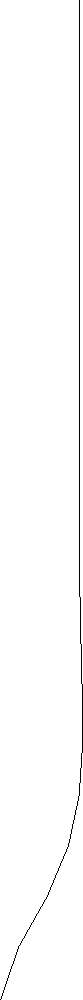
\includegraphics[height=5.5cm]{images/coque_2d_axi}
    \end{textblock*}
    \lstinputlisting[basicstyle=\ttfamily\tiny, language=gibiane, firstline=5, lastline=20]{dgibi/coque_2d_axi_3d.dgibi}
  \end{itemize}
  \vspace{1cm}
\end{frame}

\begin{frame}{\fe{Et d'autres options (2D, 1D, ...)}{And some other options (2D, 1D, ...)}}
  \begin{itemize}
    \item \fe{Exemple d'un problème de conduction stationnaire axisymétrique}
             {Example of steady state axisymmetric conduction problem}
    \begin{textblock*}{6cm}(7.2cm,-0.4cm)
      \includegraphics[width=5cm]{images/thermique_2d_axi.1}
    \end{textblock*}
    \begin{textblock*}{6cm}(6.8cm,3.5cm)
      \includegraphics[width=5cm]{images/thermique_2d_axi.2}
    \end{textblock*}
    \lstinputlisting[basicstyle=\ttfamily\tiny, language=gibiane, firstline=31, lastline=52]{dgibi/thermique_1d_2d_axi.dgibi}
  \end{itemize}
  \vspace{1cm}
\end{frame}

\begin{frame}{\fe{Et d'autres options (2D, 1D, ...)}{And some other options (2D, 1D, ...)}}
  \begin{itemize}
    \item \fe{Le même cas en 1D (cylindrique)}{The same case in 1D (cylindrical)}
    \begin{textblock*}{6cm}(7.2cm,-0.4cm)
      \includegraphics[width=5cm]{images/thermique_1d_axi.1}
    \end{textblock*}
    \begin{textblock*}{6cm}(6.8cm,3.5cm)
      \includegraphics[width=5cm]{images/thermique_1d_axi.2}
    \end{textblock*}
    \lstinputlisting[basicstyle=\ttfamily\tiny, language=gibiane, firstline=5, lastline=26]{dgibi/thermique_1d_2d_axi.dgibi}
  \end{itemize}
  \vspace{1cm}
\end{frame}




\fe{\subsection{Entrées/Sorties}}{\subsection{Inputs/Outputs}}
\begin{frame}{\fe{Lire / Sortir des données}{Reading / Writing data}}
  \begin{itemize}
    \item \fe{\kwr{SAUV}egarder au format binaire et \kwr{REST}ituer}
             {Save and Restore data in a binary file}
    \lstinputlisting[language=gibiane, firstline=40, lastline=41]{dgibi/exemples.dgibi}
    \footnotesize
    \fe{\blue{Fichier XDR}}{\blue{XDR format}}
    \normalsize
    \item \fe{Exécuter une commande \kwr{EXTE}rieure}{Run an \kwr{EXTE}rnal command}
    \lstinputlisting[language=gibiane, firstline=43, lastline=43]{dgibi/exemples.dgibi}
    \footnotesize
    \fe{\kw{tab1} contient le résultat de la commande \kw{grep}}
       {\kw{tab1} contents the output of the \kw{grep} command}
    \normalsize
    \item \fe{\kwr{ACQU}érir un fichier texte}{\kwr{ACQU}ire any text file}\\
    \footnotesize
    \fe{Lire un fichier texte, ligne par ligne}{Read a texte file, line by line}
    \lstinputlisting[language=gibiane, firstline=45, lastline=47]{dgibi/exemples.dgibi}
    \begin{textblock*}{5cm}(6.9cm,-2cm)
      \lstinputlisting[frame=single, language=gibiane, firstline=49, lastline=51]{dgibi/exemples.dgibi}
    \end{textblock*}
    \normalsize
  \end{itemize}
\end{frame}

\begin{frame}{\fe{Lire / Sortir des données}{Reading / Writing data}}
  \begin{itemize}
    \item \fe{Écrire un fichier texte (\kwr{SORT})}{Writing a text file (\kwr{SORT})}\\
    \begin{textblock*}{7cm}(5cm,0cm)
      \lstinputlisting[basicstyle=\ttfamily\tiny, frame=single, firstline=1, lastline=21]{dgibi/fibonacci.txt}
    \end{textblock*}
    \lstinputlisting[basicstyle=\ttfamily\tiny, language=gibiane, firstline=1, lastline=17]{dgibi/fibonacci.dgibi}
  \end{itemize}
\end{frame}

\begin{frame}{\fe{Lire / Sortir des données}{Reading / Writing data}}
  \begin{itemize}
    \item \fe{Lire/Écrire des \g{\blue{données tabulées}} en colonnes}
             {Read/Write \g{\blue{tabular data}} in columns}\\
    \begin{textblock*}{2cm}(9.5cm,-1cm)
      \includegraphics[width=1.5cm]{images/excel}
    \end{textblock*}
    \fe{\blue{Fichier .csv}}{\blue{.csv file}}\\
    \footnotesize
    \item[]\fe{Objets concernés : LISTENTI, LISTREEL, LISTMOTS, EVOLUTIO, TABLE}
              {Concerned objects: LISTENTI, LISTREEL, LISTMOTS, EVOLUTIO, TABLE}
    \item[]\fe{Utilisé par les éditeurs de texte ou tableur (Excel)}{Used by text editors or spreadsheet (Excel)}
    \lstinputlisting[language=gibiane, firstline=53, lastline=56]{dgibi/exemples.dgibi}
    \item[]
    \item[]\fe{Choix possible du séparateur de colonnes :}{The column separator can be changed:}
    \item[]\fe{point virgule, virgule, espace, tabulation, barre oblique...}{semicolon, comma, space, tab, slash}
  \end{itemize}
\end{frame}

\begin{frame}{\fe{Lire / Sortir des données}{Reading / Writing data}}
  \begin{itemize}
    \item \fe{Écrire des données au \g{\blue{format VTK}}}
             {Write data in \g{\blue{VTK format}}}\\
    \begin{textblock*}{3cm}(9.5cm,-0.3cm)
      \includegraphics[width=2.5cm]{images/paraview}
    \end{textblock*}
    \fe{\blue{Fichier .vtk}}{\blue{.vtk file}}\\
    \footnotesize
    \item[]\fe{Objets concernés : MAILLAGE, CHPOINT, MCHAML}
              {Concerned objects: MAILLAGE, CHPOINT, MCHAML}
    \item[]\fe{Utilisé par Paraview}{Used by Paraview}
    \lstinputlisting[language=gibiane, firstline=58, lastline=59]{dgibi/exemples.dgibi}
    \normalsize
    \item \fe{Lire/Écrire des données au \g{\blue{format MED}}}
             {Read/Write data in \g{\blue{MED format}}}\\
    \begin{textblock*}{3cm}(9.5cm,-0.6cm)
      \includegraphics[width=2.5cm]{images/salome}
    \end{textblock*}
    \begin{textblock*}{3cm}(9.5cm,0.2cm)
      \includegraphics[width=2.5cm]{images/epx}
    \end{textblock*}
    \begin{textblock*}{3cm}(9.5cm,2cm)
      \includegraphics[width=2.5cm]{images/aster}
    \end{textblock*}
    \fe{\blue{Fichier .med}}{\blue{.med file}}\\
    \footnotesize
    \item[]\fe{Objets concernés : MAILLAGE, CHPOINT, MCHAML, TABLE}
              {Concerned objects: MAILLAGE, CHPOINT, MCHAML, TABLE}
    \item[]\fe{Utilisé par Salomé, EuroPlexus, Code Aster}{Used by Salomé, EuroPlexus, Code Aster}
    \lstinputlisting[language=gibiane, firstline=61, lastline=64]{dgibi/exemples.dgibi}
    \normalsize
  \end{itemize}
\end{frame}

\begin{frame}{\fe{Développement : procédures Gibiane}{Development: Gibiane procedures}}
  \begin{itemize}
    \item \fe{Écrire chaque procédure dans un fichier texte :}
             {Write each procedure in a text file:}
    \begin{itemize}
      \item extension ".procedur"
      \item \fe{nom de fichier = nom de procédure}{file name = procedure name}
      \item \fe{1 fichier = 1 procédure}{1 file = 1 procedure}
    \end{itemize}
    \item \fe{Emplacements possibles :}{Location:}
    \begin{itemize}
      \item \kw{./}
      \item \kw{./procedur}
    \end{itemize}
    \item \fe{Lancer Cast3M comme d'habitude}{Launch Cast3M as usual}\\
    \kwr{castem24  } \kw{toto.dgibi}
    \item \fe{Idem pour les notices (fichiers ".notice")}
             {Idem for notices (manual pages) (".notice" files)}
  \end{itemize}
\end{frame}

\begin{frame}{\fe{Développement : sources Esope}{Development: Esope sources}}
  \begin{itemize}
    \item \fe{L'utilisateur peut modifier/corriger/ajouter le code source des opérateurs et directives}
             {The user can modify/correct/add the source code of operators and directives}
    \item \fe{Compilation des fichiers source Esope}{Compilation of Esope source files}\\
    \kwr{compilcast24  } \kw{toto.eso titi.eso ...}
    \item \fe{Édition des liens}{Linking}\\
    \kwr{essaicast24}\\
    \fe{$\Rightarrow$ création d'un fichier exécutable binaire : \g{\kwg{cast\_24}}}
       {$\Rightarrow$ creation of a binary executable file: \g{\kwg{cast\_24}}}\\
       \fe{$\Rightarrow$ version locale de Cast3M}
          {$\Rightarrow$ local version of Cast3M}
    \item \fe{Lancer Cast3M comme d'habitude}{Launch Cast3M as usual}\\
    \kwr{castem24  } \kw{toto.dgibi}
  \end{itemize}
\end{frame}

\begin{frame}{\fe{Et pour finir}{And to complete}}
  \begin{itemize}
    \item \fe{Consulter la \g{\blue{documentation}} régulièrement}
             {Peruse \g{\blue{documentation}} regularly}\\
    \footnotesize
    \fe{$\sim$ 70 instructions découvertes durant cette formation\\
        près de 1400 instructions existantes !}
       {$\sim$ 70 instructions reviewed during this course\\
        around 1400 available instructions!}\\~
    \normalsize
    \item \fe{Inscription à la \g{\blue{liste de diffusion Cast3M}} (voir le site web Cast3M)}
             {Subscription to the \g{\blue{Cast3M mailing list}} (see the Cast3M web site)}\\
    \footnotesize
    \fe{Envoyer un e-mail vide à \href{mailto:sympa@umontpellier.fr}{\kw{sympa@umontpellier.fr}}\\
        avec comme objet du message :}
       {Send an e-mail at \href{mailto:sympa@umontpellier.fr}{\kw{sympa@umontpellier.fr}}\\
        with in the message frame:}
    \begin{center}
      \kw{SUB  cast3m-util last\_name  first\_name}
    \end{center}
    \fe{et rien d'autre ! (pas de message, pas de signature, …)}
       {and nothing more! (no object, no signature, …)}\\~
    \normalsize
    \item \fe{\g{\blue{Club Cast3M}} : séminaire annuel des utilisateurs}
             {\g{\blue{Club Cast3M}}: annual users seminar}\\
    \footnotesize
    \fe{Chaque année en novembre dans le sud de Paris\\
        Présentation de travaux réalisés avec Cast3M, nouveautés de la prochaine version\\
        Inscription gratuite !}
       {Each year in November in the south of Paris\\
        Presentation of studies performed with Cast3M, developments in the next release\\
        Free registration!}
  \end{itemize}
\end{frame}



\end{document}
